%%%%%%%%%%%%%%%%%%%%%%%%%%
%% T A G    M E M O R Y %%
%%%%%%%%%%%%%%%%%%%%%%%%%%

\subsection{Tag Memory}
\label{subsec:tag_memory}

The Tag Memory block encapsulates the multi-bank memory used to store cache tags and valid bits. Each bank stores the tag and valid bit corresponding to a specific way across all cache sets.

\begin{figure}[H]
	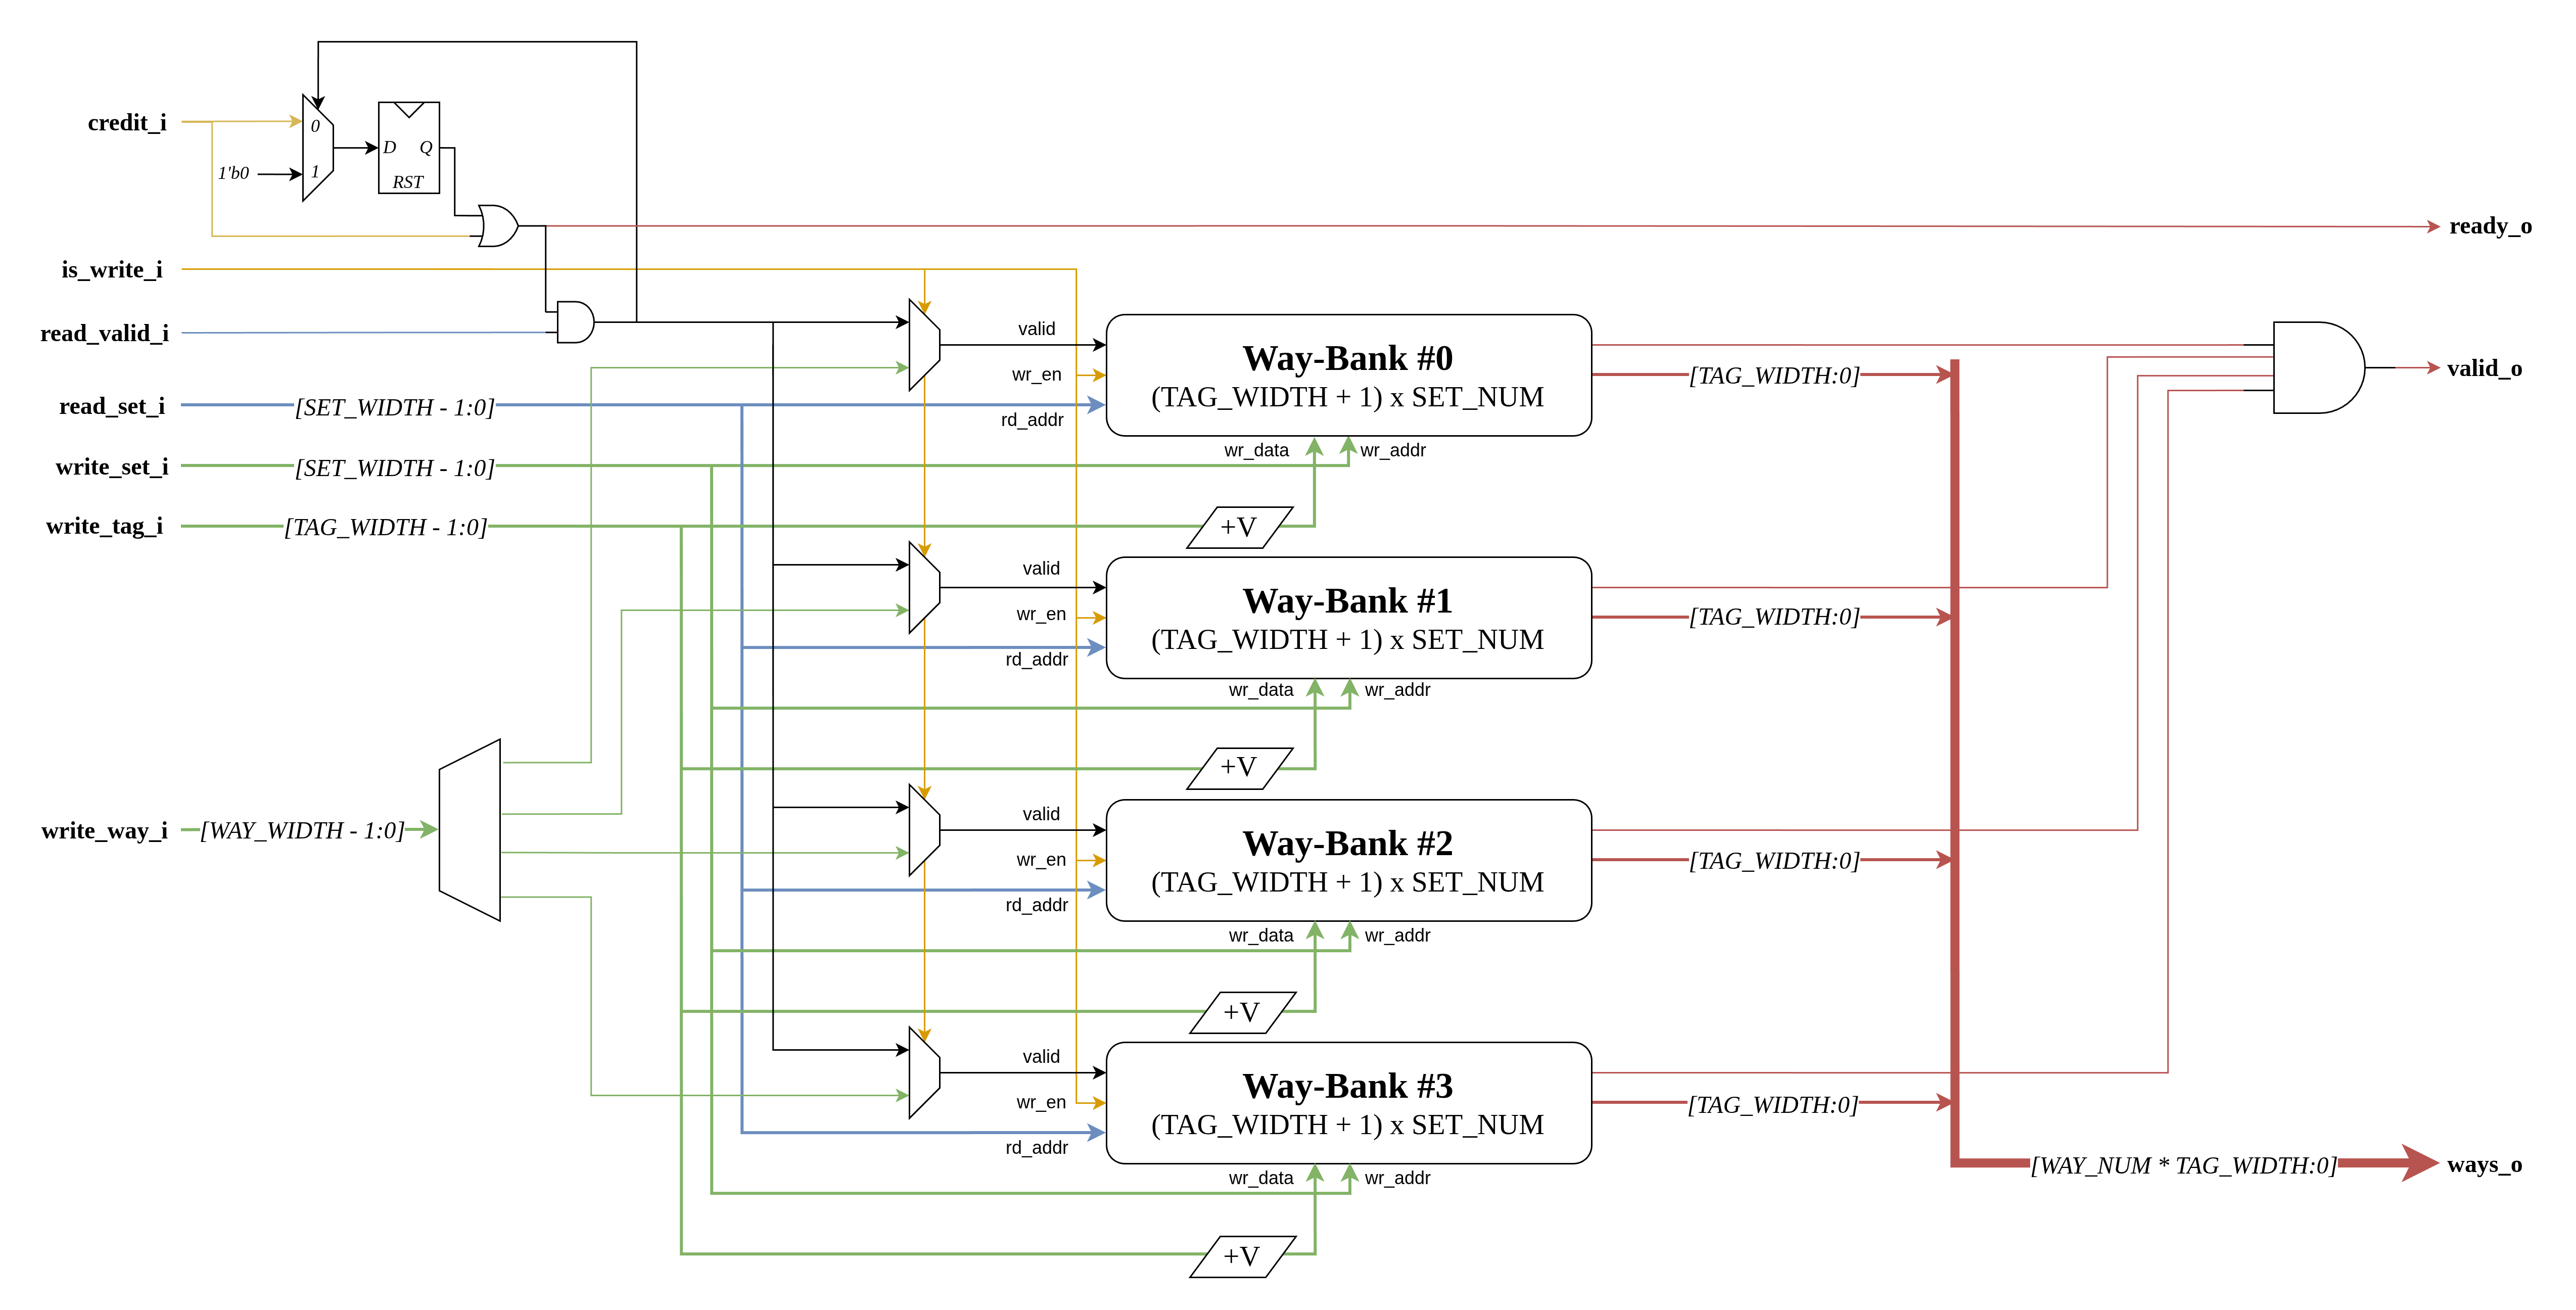
\includegraphics[width=16cm]{Tag_Memory.png}
	\caption{Tag Memory scheme (4-way cache)}
\end{figure}

Each memory bank is implemented as a pseudo-dual-port memory with a single memory access port that can be used for either a read or a write operation. Read requests are issued by the CPU-side cache logic, while write requests are generated by the cache control logic during cache operations. The access type is selected according to the current cache operation.

The Tag Memory also contains a credit counter that stores a single credit. A read request consumes the available credit, preventing a new read operation from being started until the current cache access has been completed. The credit is restored when the requested data is found in the cache or when a valid response is received from the external memory through the AXI4-Lite \verb|R| or \verb|B| channel. A restored credit can be used in the same clock cycle.

Write operations do not consume the credit and can therefore be performed independently of the credit counter.

Both read and write operations have a latency of one clock cycle.

\begin{table}[H]
	\centering
	\small
	\begin{tabularx}{\textwidth}{l c c X}
		\toprule
		\textbf{Parameter} & \textbf{Valid Range} & \textbf{Default} & \textbf{Description} \\
		\midrule
		
		\verb|TAG_WIDTH| &
		Positive integer &
		--- &
		Width of the tag stored in each cache line. \\
		
		\verb|WAY_NUM| &
		Power of 2 &
		--- &
		Number of cache ways. \\
		
		\verb|SET_NUM| &
		Power of 2 &
		--- &
		Number of cache sets. \\
		
		\bottomrule
	\end{tabularx}
	\caption{Tag Memory parameters}
	\label{tab:tag_memory_parameters}
\end{table}

\begin{table}[htbp]
	\centering
	\label{tab:tag_memory_ports}
	\small
	\begin{tabularx}{\textwidth}{l c c X}
		\toprule
		\textbf{Ports} & \textbf{Direction} & \textbf{Width} & \textbf{Description} \\
		\midrule
		\verb| read_valid_i | & Input & \verb| 1 | & Indicates a valid read request. \\
		\verb| read_set_i | & Input & \verb| SET_WIDTH | & Index of the cache set to be read. \\
		\verb| write_set_i | & Input & \verb| SET_WIDTH | & Index of the cache set to which the tag is written. \\
		\verb| write_tag_i | & Input & \verb| TAG_WIDTH | & Tag to be written to the selected cache line. \\
		\verb| write_way_i | & Input & \verb| WAY_WIDTH | & Index of the way in which the tag is stored. \\
		\verb| credit_i | & Input & \verb| 1 | & Indicates that a credit is available for a read request. \\
		\verb| ready_o | & Output & \verb| 1 | & Indicates readiness for a read request accept. \\
		\verb| valid_o | & Output & \verb| 1 | & Indicates that valid output data is available. \\
		\verb| ways_o | & Output & \verb| (TAG_WIDTH + 1) * WAY_NUM | & Tags and valid bits stored in requested cache set. \\
		\bottomrule
	\end{tabularx}
	\caption{Tag Memory ports}
\end{table}